% Overleaf-ready documentation for MeshPay over Mininet-WiFi
\documentclass[11pt,a4paper]{article}

\usepackage[margin=1in]{geometry}
\usepackage[T1]{fontenc}
\usepackage{lmodern}
\usepackage{hyperref}
\usepackage{xcolor}
\usepackage{graphicx}
\usepackage{amsmath, amssymb}
\usepackage{enumitem}
\usepackage{listings}
\usepackage{tikz}
\usetikzlibrary{positioning, arrows.meta, shapes.multipart, calc}
\usepackage{msc} % Message Sequence Charts

\hypersetup{
  colorlinks=true,
  linkcolor=blue,
  urlcolor=blue,
  citecolor=blue
}

\title{MeshPay over Mininet-WiFi\\Implementation Documentation}
\author{Project Documentation}
\date{\today}

\lstset{
  basicstyle=\ttfamily\small,
  keywordstyle=\bfseries\color{teal!60!black},
  commentstyle=\itshape\color{gray!70!black},
  stringstyle=\color{purple!60!black},
  showstringspaces=false,
  frame=single,
  breaklines=true,
  tabsize=2,
}

\begin{document}
\maketitle
\tableofcontents
\vspace{1em}

\section{Overview}
MeshPay is an offline-first payment simulation built atop \emph{Mininet-WiFi}. It models a network of:\\
\begin{itemize}[noitemsep]
  \item \textbf{Authorities} (committee validators)\,
  \item \textbf{Clients} (end-users), and
  \item an optional \textbf{Gateway + HTTP Bridge} for web integrations.
\end{itemize}

Networking is simulated using IEEE 802.11s mesh links with channel/propagation handled via \texttt{wmediumd}. Application messages use pluggable transports (TCP, UDP, Wi-Fi Direct) executed \emph{inside} each station namespace to ensure realistic connectivity in simulation.

\paragraph{Key packages}
\begin{itemize}[noitemsep]
  \item \texttt{meshpay/types.py}: Core domain dataclasses and enums
  \item \texttt{meshpay/messages.py}: Message DTOs and JSON (de)serialisation
  \item \texttt{meshpay/nodes/authority.py}: Authority node logic
  \item \texttt{meshpay/nodes/client.py}: Client node logic
  \item \texttt{meshpay/transport/*}: TCP, UDP, Wi-Fi Direct transports
  \item \texttt{meshpay/api/gateway.py}: Gateway for forwarding
  \item \texttt{meshpay/api/bridge.py}: HTTP bridge server
  \item \texttt{meshpay/cli_fastpay.py}: Interactive CLI
  \item \texttt{meshpay/examples/meshpay_demo.py}: Demo topology
  \item \texttt{meshpay/logger/*}: Lightweight terminal/file loggers
\end{itemize}

\section{High-level Architecture}
\begin{center}
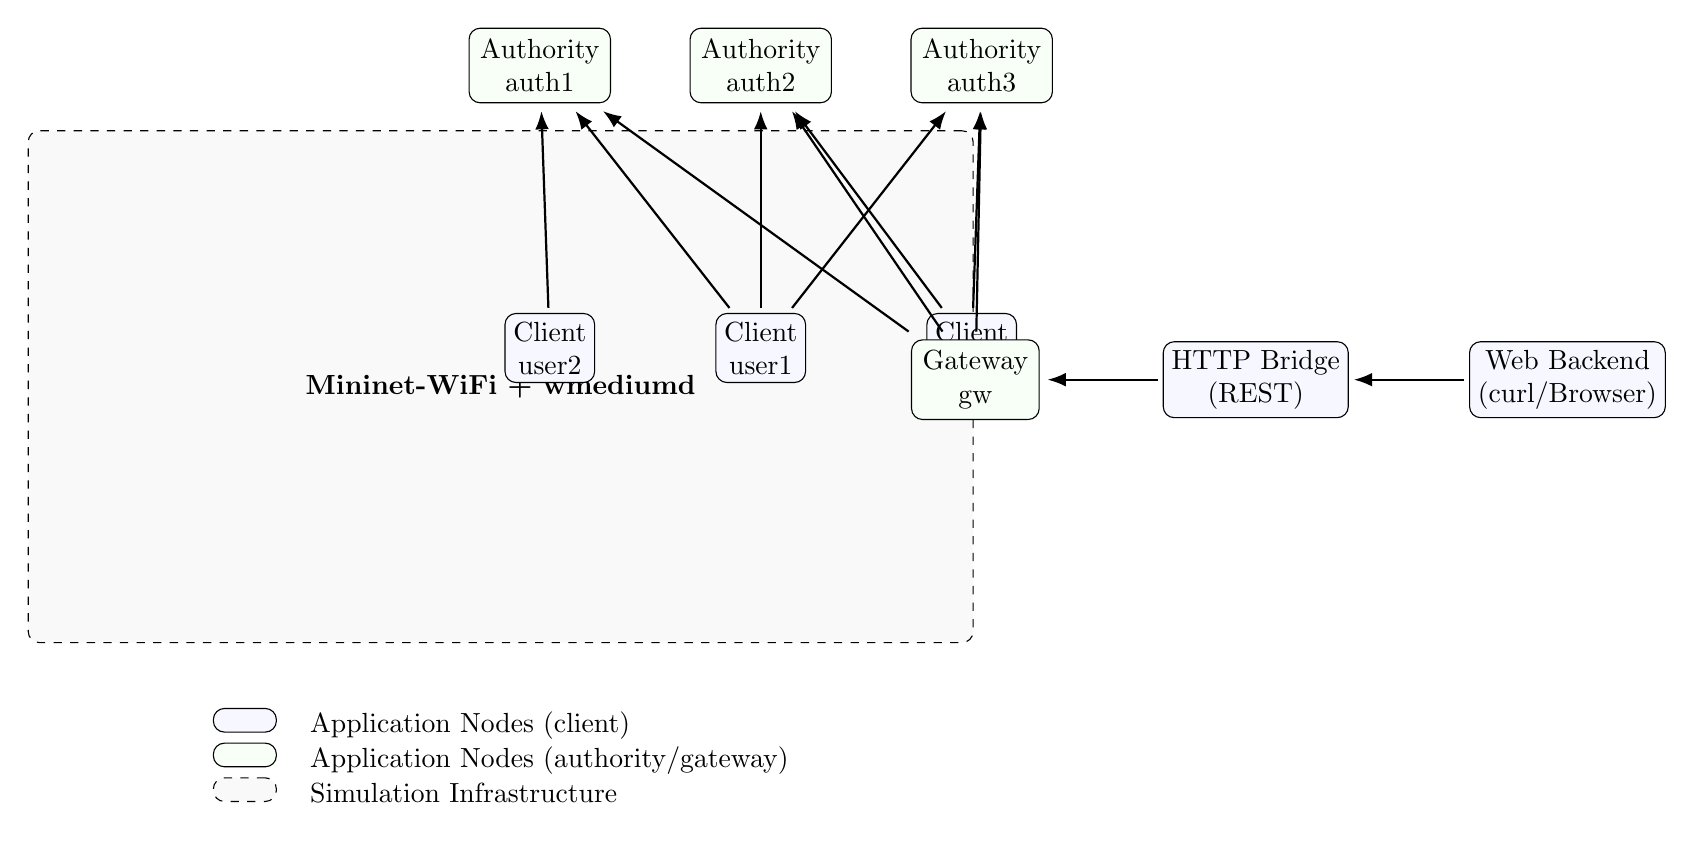
\begin{tikzpicture}[
  node distance=18mm,
  box/.style={draw, rounded corners, align=center, inner sep=3pt, outer sep=2pt, fill=blue!3},
  comp/.style={draw, rounded corners, align=center, inner sep=4pt, outer sep=3pt, fill=green!3},
  infra/.style={draw, dashed, rounded corners, align=center, inner sep=4pt, outer sep=3pt, fill=gray!5},
  arr/.style={-Latex, thick}
]

% Infra box
\node[infra, minimum width=12cm, minimum height=6.5cm] (wifi) {\textbf{Mininet-WiFi + wmediumd}};

% Authorities cluster
\node[comp, above left=35mm and -15mm of wifi.center] (auth1) {Authority\\auth1};
\node[comp, right=8mm of auth1] (auth2) {Authority\\auth2};
\node[comp, right=8mm of auth2] (auth3) {Authority\\auth3};

% Clients
\node[box, below=25mm of auth2] (c1) {Client\\user1};
\node[box, left=14mm of c1] (c2) {Client\\user2};
\node[box, right=14mm of c1] (c3) {Client\\user3};

% Gateway + Bridge
\node[comp, below right=28mm and -20mm of auth3] (gw) {Gateway\\gw};
\node[box, right=14mm of gw] (bridge) {HTTP Bridge\\(REST)};

% External Web
\node[box, right=14mm of bridge] (web) {Web Backend\\(curl/Browser)};

% Mesh links (conceptual)
\draw[arr] (c1) -- (auth1);
\draw[arr] (c1) -- (auth2);
\draw[arr] (c1) -- (auth3);
\draw[arr] (c2) -- (auth1);
\draw[arr] (c3) -- (auth2);
\draw[arr] (c3) -- (auth3);

% Gateway links
\draw[arr] (gw) -- (auth1);
\draw[arr] (gw) -- (auth2);
\draw[arr] (gw) -- (auth3);
\draw[arr] (bridge) -- (gw);
\draw[arr] (web) -- (bridge);

% Legend
\node[below=6mm of wifi.south] (legend) {
  \begin{tabular}{ll}
    \tikz \node[box, minimum width=8mm, minimum height=3mm]{}; & Application Nodes (client) \\
    \tikz \node[comp, minimum width=8mm, minimum height=3mm]{}; & Application Nodes (authority/gateway) \\
    \tikz \node[infra, minimum width=8mm, minimum height=3mm]{}; & Simulation Infrastructure \\
  \end{tabular}
};

\end{tikzpicture}
\end{center}

\section{End-to-end Flow (Sequence)}
\begin{center}
\begin{msc}{FastPay Transfer}
  \setlength{\instdist}{3.5cm}
  \declinst{client}{Client}{userX}
  \declinst{authA}{Authority}{authA}
  \declinst{authB}{Authority}{authB}
  \declinst{gateway}{Gateway}{gw}

  % Client initiates
  \mess{TRANSFER\_REQUEST}{client}{authA}
  \mess{TRANSFER\_REQUEST}{client}{authB}

  % Authorities respond
  \mess{TRANSFER\_RESPONSE (ok/err)}{authA}{client}
  \mess{TRANSFER\_RESPONSE (ok/err)}{authB}{client}

  % Quorum (client-side check)
  \action*{Client counts certificates; if quorum reached, build CONFIRMATION\_ORDER}{client}

  % Confirmation broadcast via Gateway (optional)
  \mess{CONFIRMATION\_REQUEST}{client}{gateway}
  \mess{CONFIRMATION\_REQUEST}{gateway}{authA}
  \mess{CONFIRMATION\_REQUEST}{gateway}{authB}

  \action*{Authorities apply state changes (balances, sequences)}{authA}
  \action*{Authorities apply state changes (balances, sequences)}{authB}
\end{msc}
\end{center}

\section{Modules and Implementation Details}
This section provides a practical summary of each module. Class and function names refer to the code under \texttt{meshpay/}.

\subsection{types.py}
\textbf{Purpose}: Domain model for MeshPay.\\
\textbf{Key dataclasses and enums}:
\begin{itemize}[noitemsep]
  \item \texttt{NodeType}: \texttt{AUTHORITY|CLIENT|GATEWAY}
  \item \texttt{TransactionStatus}: \texttt{PENDING|CONFIRMED|REJECTED|FINALIZED}
  \item \texttt{Address}: Logical node address (id, IP, port, type)
  \item \texttt{TransferOrder}: Client-issued transfer intent
  \item \texttt{SignedTransferOrder}: Authority sign-off for a transfer
  \item \texttt{ConfirmationOrder}: Committee-level confirmation package
  \item \texttt{TokenBalance}, \texttt{AccountOffchainState}, \texttt{AuthorityState}, \texttt{ClientState}, \texttt{GatewayState}
\end{itemize}
\textbf{Notes}:\ \texttt{\_\_post\_init\_\_} methods ensure timestamps, UUIDs, and robust deserialisation from JSON.

\subsection{messages.py}
\textbf{Purpose}: Message DTOs and JSON helpers.\\
\textbf{Key types}:
\begin{itemize}[noitemsep]
  \item \texttt{MessageType}: TRANSFER\_REQUEST/RESPONSE, CONFIRMATION\_REQUEST/RESPONSE, SYNC, PEER\_DISCOVERY, HEARTBEAT, ERROR
  \item \texttt{Message}: Base envelope (id, type, sender, recipient, timestamp, payload)
  \item \texttt{TransferRequestMessage}, \texttt{TransferResponseMessage}
  \item \texttt{ConfirmationRequestMessage}, \texttt{SyncRequestMessage}, \texttt{PeerDiscoveryMessage}
\end{itemize}
\textbf{Notes}:\ JSON serialisation uses dataclass \texttt{asdict} and explicit enum/UUID conversions.

\subsection{nodes/authority.py}
\textbf{Purpose}: Authority node behaviour (extends Mininet-WiFi \texttt{Station}).\\
\textbf{Highlights}:
\begin{itemize}[noitemsep]
  \item Transport selection (TCP/UDP/Wi-Fi Direct) with \texttt{start\_fastpay\_services()}
  \item In-memory queues and background threads for message handling
  \item Validation helpers for transfer and confirmation orders
  \item Optional periodic blockchain sync hooks
  \item Performance metrics via \texttt{MetricsCollector}
\end{itemize}
\textbf{Key methods}: \texttt{handle\_transfer\_order()}, \texttt{handle\_confirmation\_order()}, \texttt{get\_account\_balance()}, \texttt{get\_performance\_stats()}.

\subsection{nodes/client.py}
\textbf{Purpose}: Client node behaviour (extends \texttt{Station}).\\
\textbf{Highlights}:
\begin{itemize}[noitemsep]
  \item Builds \texttt{TransferOrder}, wraps into \texttt{Message} and broadcasts to authorities
  \item Tracks sent certificates, pending orders, and local sequence number
  \item Validates responses and constructs \texttt{ConfirmationOrder} on quorum
\end{itemize}
\textbf{Key methods}: \texttt{transfer()}, \texttt{handle\_transfer\_response()}, \texttt{broadcast\_confirmation()}.

\subsection{transport/ (TCP, UDP, Wi-Fi Direct)}
\textbf{Purpose}: Pluggable transports implementing a common \texttt{NetworkTransport} protocol.\\
\textbf{Design}: All network I/O is executed \emph{inside} the station namespace using \texttt{node.cmd(...)} to run small Python scripts (servers/clients). This mirrors realistic connectivity in a Mininet-WiFi simulation.
\begin{itemize}[noitemsep]
  \item \texttt{tcp.py} (\textbf{TCPTransport}): in-namespace TCP server; monitor thread tails a log file to deliver messages to the application queue.
  \item \texttt{udp.py} (\textbf{UDPTransport}): UDP server and sender; background log-tail + deserialisation.
  \item \texttt{wifiDirect.py} (\textbf{WiFiDirectTransport}): alias subclass of TCPTransport for Wi-Fi Direct topologies.
  \item \texttt{transport.py}: \textbf{TransportKind} enum and \textbf{NetworkTransport} protocol.
\end{itemize}

\subsection{api/gateway.py}
\textbf{Purpose}: Stateless forwarder between clients and authorities.\\
\textbf{Highlights}: Maintains authority registry, forwards transfer/confirmation requests, and produces per-authority result summaries. Intended to be bound to interfaces in topologies that link the gateway with each authority.

\subsection{api/bridge.py}
\textbf{Purpose}: Minimal HTTP server exposing REST endpoints for web backends.\\
\textbf{Endpoints} (examples): \texttt{/authorities}, \texttt{/network/metrics}, \texttt{/transfer}, \texttt{/confirm}, \texttt{/shards}, \texttt{/accounts/<addr>}.

\subsection{cli\_fastpay.py}
\textbf{Purpose}: Interactive CLI built on Mininet-WiFi CLI, adding FastPay commands.\\
\textbf{Commands}: \texttt{balance}, \texttt{transfer}, \texttt{infor}, \texttt{voting\_power}, \texttt{performance}, \texttt{broadcast\_confirmation}, \texttt{update\_onchain\_balance}.

\subsection{examples/meshpay\_demo.py}
\textbf{Purpose}: Creates an IEEE 802.11s mesh topology with optional Internet gateway and NAT, configures links, starts services, and launches the CLI.
\begin{itemize}[noitemsep]
  \item Uses \texttt{Mininet\_wifi(link=wmediumd, wmediumd\_mode=interference)}
  \item Builds authorities, clients, and optional gateway, then links them with \texttt{mesh}
  \item Seeds demo balances and starts transports
\end{itemize}

\subsection{logger/*}
\textbf{Purpose}: Simple per-node loggers that write to \texttt{/tmp} and can spawn \texttt{xterm} tails for live viewing. Classes: \texttt{AuthorityLogger}, \texttt{ClientLogger}, \texttt{BridgeLogger}.

\section{Error Handling and Robustness}
\begin{itemize}[noitemsep]
  \item Transport connection failures are logged and cause service start to return \texttt{False}.
  \item JSON parsing errors in bridges/servers return structured error responses.
  \item Type conversions (UUIDs, enums) are validated when deserialising messages and orders.
\end{itemize}

\section{Configuration and Environment}
Configuration lives under \texttt{mn\_wifi/services/core/config.py} (e.g., supported tokens, sync intervals). Demo scripts print helpful run-time logs. For web testing, the bridge exposes HTTP endpoints reachable within the simulated network.

\section{Running the Demo}
\begin{lstlisting}[language=bash]
# From repository root, run with sudo due to network namespaces
sudo PYTHONPATH=$(pwd) python3 -m meshpay.examples.meshpay_demo --authorities 3 --clients 2

# Enable Internet gateway + HTTP bridge
sudo PYTHONPATH=$(pwd) python3 -m meshpay.examples.meshpay_demo --authorities 3 --clients 2 --internet --gateway-port 8080

# After startup, try bridge endpoints from inside the simulation
# Example (if gateway is at 10.0.0.254):
curl http://10.0.0.254:8080/authorities
curl http://10.0.0.254:8080/shards
\end{lstlisting}

\section{Diagrams: Implementation Internals}
\subsection{Authority State Update Flow}
\begin{center}
\begin{tikzpicture}[
  node distance=8mm,
  box/.style={draw, rounded corners, align=left, inner sep=3pt, outer sep=2pt, fill=yellow!10},
  arr/.style={-Latex, thick}
]
\node[box] (recv) {Receive TRANSFER\_REQUEST\\(\texttt{_process\_message})};
\node[box, below=of recv] (validate) {Validate order\\(balance, seq, token)};
\node[box, below=of validate] (pending) {Set pending confirmation\\and sign order};
\node[box, below=of pending] (metrics) {Record transaction metric};
\node[box, below=of metrics] (respond) {Respond TRANSFER\_RESPONSE};

\draw[arr] (recv) -- (validate);
\draw[arr] (validate) -- (pending);
\draw[arr] (pending) -- (metrics);
\draw[arr] (metrics) -- (respond);
\end{tikzpicture}
\end{center}

\section{Testing and Extensibility}
\begin{itemize}[noitemsep]
  \item Transports can be extended by implementing the \texttt{NetworkTransport} protocol.
  \item Additional message types can be added to \texttt{MessageType} and corresponding DTOs.
  \item The gateway/bridge can be expanded with authentication and richer response aggregation.
\end{itemize}

\section{Notes on Simulation Specifics}
\begin{itemize}[noitemsep]
  \item All network scripts run within station namespaces via \texttt{node.cmd()}, ensuring IP reachability.
  \item Mesh links and propagation use \texttt{wmediumd} in interference mode; ranges and channel settings affect connectivity.
  \item For visualising logs, the logger classes can spawn \texttt{xterm} windows tailing files under \texttt{/tmp}.
\end{itemize}

\section{Appendix: Key Files Reference}
\begin{itemize}[noitemsep]
  \item \texttt{meshpay/types.py} – Domain types
  \item \texttt{meshpay/messages.py} – Message DTOs
  \item \texttt{meshpay/nodes/authority.py} – Authority node
  \item \texttt{meshpay/nodes/client.py} – Client node
  \item \texttt{meshpay/transport/tcp.py} – TCP transport
  \item \texttt{meshpay/transport/udp.py} – UDP transport
  \item \texttt{meshpay/transport/wifiDirect.py} – Wi-Fi Direct alias transport
  \item \texttt{meshpay/api/gateway.py} – Gateway forwarder
  \item \texttt{meshpay/api/bridge.py} – HTTP bridge
  \item \texttt{meshpay/cli_fastpay.py} – Interactive CLI
  \item \texttt{meshpay/examples/meshpay_demo.py} – Demo topology
\end{itemize}

\end{document}
